\usetikzlibrary{calc}
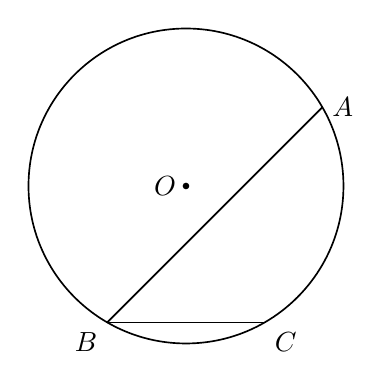
\begin{tikzpicture}[x=1cm,y=1cm,line width=.6pt,font=\normalsize]
\coordinate (O) at (0,0);
\coordinate (A) at (1.7321,1.0);
\coordinate (B) at (-1.0,-1.7321);
\coordinate (C) at (1.0,-1.7321);
\draw (O) circle[radius=2cm];
\draw (B)--(A);
\draw (B)--(C);
\fill (O) circle[radius=1.2pt];
\node[left] at (O) {$O$};
\node[right] at (A) {$A$};
\node[below left] at (B) {$B$};
\node[below right] at (C) {$C$};
\end{tikzpicture}
